% !TEX encoding = UTF-8
% !TEX TS-program = pdflatex
% !TEX root = ../tesi.tex

%**************************************************************
\chapter{Homepage: le 6 W}
\label{cap:le 6 w}
Nelle sezioni seguenti vengono analizzate le cosiddette 6 W, partendo dalla Homepage e poi analizzando le altre pagine del sito. Due di esse ("Mercatino" e "I Nostri Atleti") sono ancora in costruzione al momento in cui ho fatto l'analisi del sito e pertanto non verranno prese in considerazione.

%**************************************************************
\begin{figure}[H]
    \centering
    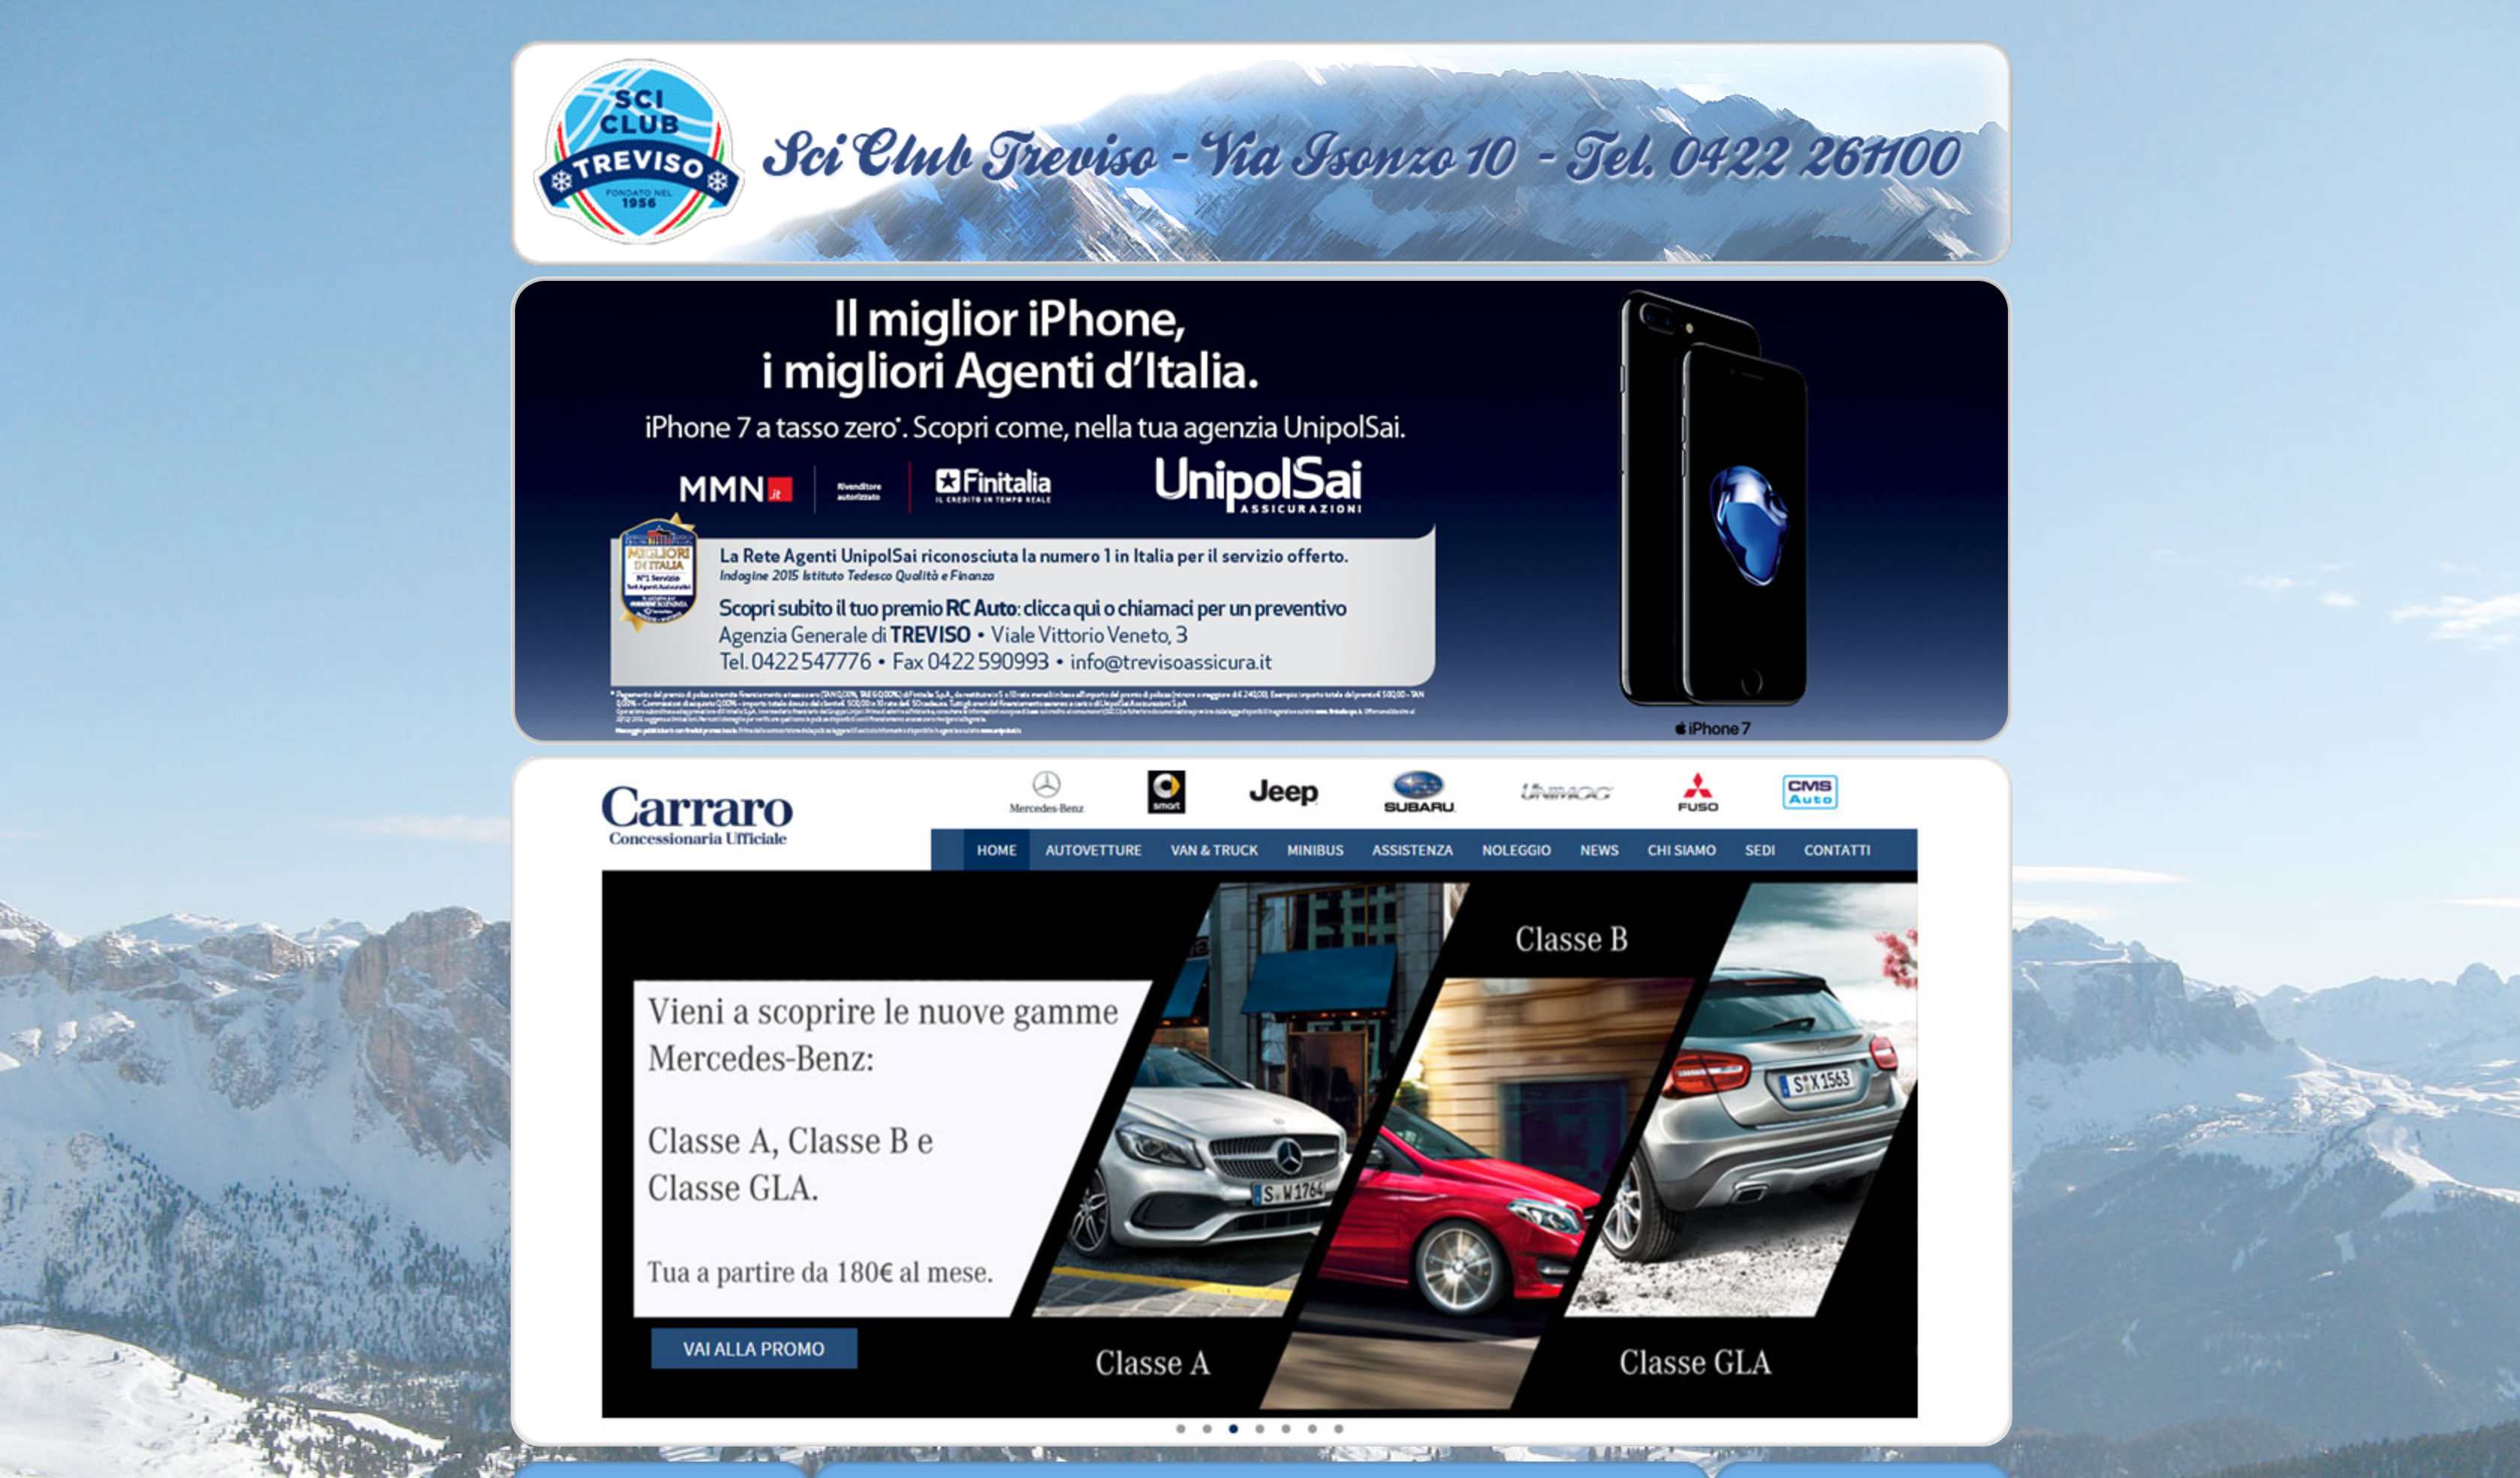
\includegraphics[scale=0.2]{./immagini/homepage}
    \caption [Homepage del sito]{Homepage del sito \siteName}
\end{figure}

La prima pagina che si vede quando si visita il sito è la Homepage (ovviamente). Tuttavia questa pagina è tutto tranne che una homepage: dovrebbe essere il cuore del sito e deve essere gestita come un testo giornalistico, quindi deve rispettare le 6W. Ciò che vede l'utente quando entra sono due grandi banner pubblicitari: il "vero" sito inizia dopo uno scroll di una pagina. Per poter rispondere (in parte) alle 6 W è necessario quindi scrollare di una pagina. \\

\begin{figure}[H]
    \centering
        \subfloat[Homepage dopo uno scroll]{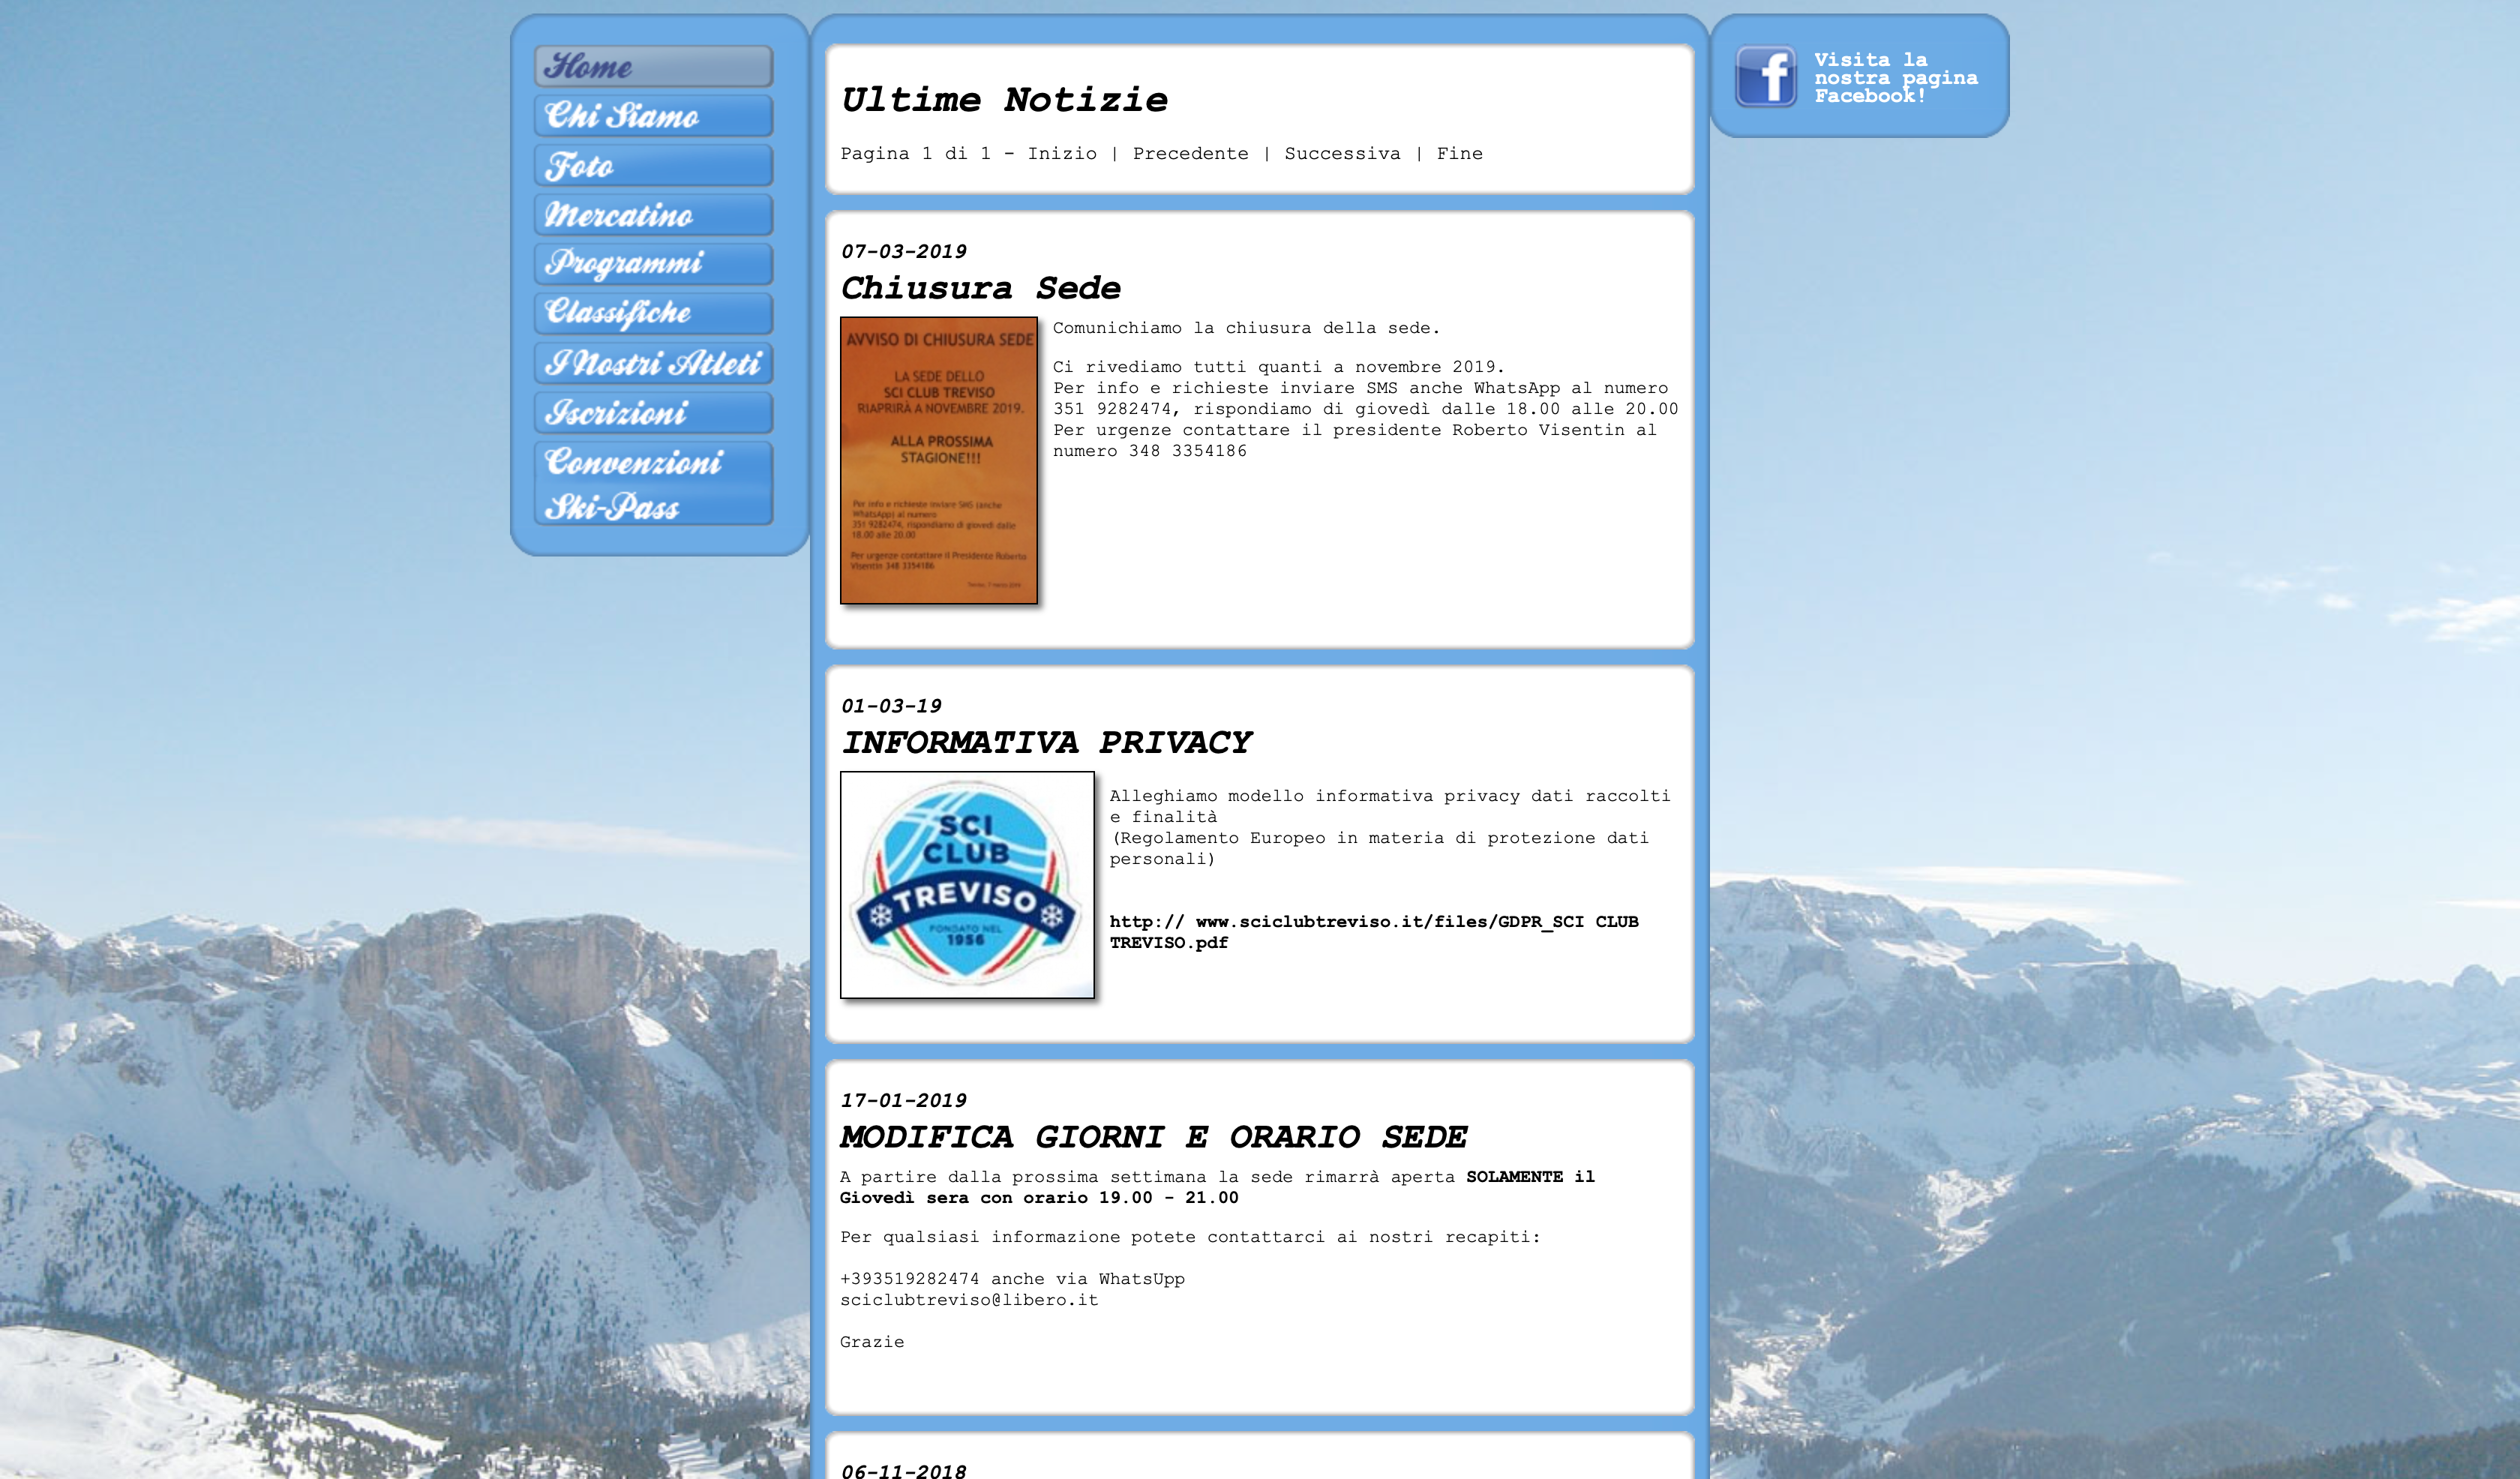
\includegraphics[width=0.4\columnwidth]{./immagini/homepage2}}
        \qquad
		\subfloat[Homepage dopo due  scroll]{\includegraphics[width=0.4\columnwidth]{./immagini/homepage3}}
	\caption [Homepage del sito]{Homepage del sito \siteName}
\end{figure}

Da qui si può iniziare a vedere il sito vero e proprio anche se l'organizzazione e le informazione presenti nella Homepage sono poste in modo sbagliato.

\begin{wrapfigure}{l}{0.4\textwidth}
	\vspace{-20pt}
	\begin{center}
	  \includegraphics[width=0.2 \textwidth]{./immagini/menu}
	\end{center}
	\vspace{-20pt}
	\caption[Menù del sito]{Menù del sito}
	\vspace{-70pt}
\end{wrapfigure}
\paragraph{Menù}
Una grave carenza del sito, a mio avviso, è il menù che non resta fermo nella finestra, obbligando l'utente a tornare all'inizio della pagina per navigare nel sito. Sarebbe stato meglio tenerlo fisso in alto alla pagina oppure mettere a disposizione un pulsante che permetta di ritornare all'inizio. Inoltre il font troppo sofisticato utilizzato in esso, rende difficile la lettura delle varie voci.
\vspace{40pt}

    \section{Where}
        \begin{center}
            \textit{"A che tipo di sito sono arrivato?"}
        \end{center}
        Dalla Homepage è difficile capire a che tipo  di  sito si è arrivati, in quando l'unica informazione riguardante il sito è il logo e il nome dell'associazione in alto al centro. Come si può notare dalla figura 2.1, non vi sono altre informazione se non pubblicitarie, cosa che non aiuta l'utente a capire a che sito è arrivato.
         
    \section{Who}
        \begin{center}
            \textit{"Chi rappresenta il sito?"}
        \end{center}
        Vale quanto detto per l'asse "Where": si capisce di essere nel sito dello Sci Club Treviso grazie ad un'immagine contente il logo e il nome dell'associazione, posta nella parte superiore della pagina, ma i due banner pubblicitari di due sponsor dell'associazione, fanno pensare diversamente. La prima volta che ho visitato questo sito pensavo di essere capitato nel sito sbagliato, dato che l'unica cosa che vedevo erano le pubblicità e non vi è alcuna altra informazione. 

    \section{Why}
    \begin{center}
        \textit{"Perché mai dovrei fermarmi su questo sito?"}
    \end{center}
    Nel sito non presenta una sezione dove descrive cosa esso rappresenta, ma da per scontato che l'utente sappia esattamente dove sia arrivato e del perché si trovi lì. Questo potrebbe essere in parte vero, perché un utente iscritto all'associazione Sci Club Treviso potrebbe avere la necessità di consultare alcune informazione presenti, ma un utente non iscritto che visita il sito, potrebbe non sapere che quello è il sito che cerca a causa (di nuovo) della pubblicità posta nel posto sbagliato.

    \section{What}
    \begin{center}
        \textit{"Cosa offre il sito?”}
    \end{center}
    A prima vista, ciò che offre il sito sembrerebbe essere la vendita di automobili o di telefoni. Solo scorrendo nella pagina  si trovano alcune informazione riguardanti l'associazione, ma queste sono poste in forma di  elenco senza una correlazione logica tra loro. Inoltre spesso rimandano ad altre pagine del sito senza fornire un link diretto ma solo specificando il nome della pagina da visitare.

    \section{When}
    \begin{center}
        \textit{"Quali sono le ultime novità?”}
    \end{center}
    Questo è l'unico asse abbastanza soddisfatto: la homepage presenta un elenco delle ultime novità che riguardano l'associazione, anzi la homepage è costituita interamente dalle ultime notizie (e dalla pubblicità). Le novità sono ordinate per data di pubblicazione e non per  aree tematiche, di conseguenza l'utente che ricerca una particolare informazione sarà costretto a scorrere tutta la pagina.

    \section{How}
    \begin{center}
        \textit{"Come faccio ad arrivare alle sezioni principali?”}
    \end{center}
    Un menù posto sulla sinistra sotto i banner pubblicitari, permette all'utente di navigare all'interno del sito. La mancanza di un box di ricerca è una grave carenza, perché spesso l'utente non sa cosa cercare e soprattutto dove.
    
